\documentclass[12pt,a4paper]{article}
\usepackage{nopageno}
\usepackage[polish]{babel}
\usepackage[T1]{fontenc}
\usepackage[utf8]{inputenc}
\usepackage{amsmath,amsfonts}
\usepackage{titling}
\usepackage{mathtools}
\usepackage[margin=0.6in]{geometry} 
\usepackage{graphicx}
\usepackage{tikz}

\title{MDL Lista 10}
\author{Cezary Świtała}

\begin{document}
\maketitle

\noindent
\textbf{Zadanie 1} Przypuśćmy, że w grafie \(G\) wszystkie wagi krawędzi są różne. Pokaż, nie używając żadnego algorytmu, że \(G\) zawiera tylko jedno minimalne drzewo rozpinające.
\vskip 0.5cm

Załóżmy nie wprost, że istnieją dwa różne drzewa MST \(T_1\) i \(T_2\). Ze zbioru krawędzi, które są tylko w jednym z drzew -- \(E'\), wybierzmy tą o najmniejszej wadze, nazwijmy ją \(e_1\). Wiemy, że taka istnieje gdyż oba drzewa są opisane na tych samych wierzchołkach, ale są różne, czyli muszą różnić się krawędzią. Bez straty ogólności możemy założyć, że \( e_1 \in T_1 \).

Jeśli dodamy \(e_1\) do \(T_2\) to otrzymamy w nim cykl, gdyż otrzymany graf nie jest drzewem, bo ma \(n\) krawędzi, ale jest to graf spójny, czyli musi być cykliczny (inaczej by był drzewem). Na cyklu musi znajdować się jakaś krawędź, która nie należy do \(T_1\), inaczej \(T_1\) miałoby cykl, a nie ma bo jest drzewem, nazwiemy ją \(e_2\). Skoro krawędź ta należy tylko do jednego drzewa, to należy też do zbioru \(E'\) i skoro nie była krawędzią o najmniejszej wadze, to \(c(e_1) < c(e_2)\).

Tworzymy zatem nowy graf dokładając do drzewa \(T_2\) krawędź \(e_1\) i usuwając \(e_2\). Nie tracimy spójności, gdyż krawędź \(e_2\) leżała na cyklu, a żaden most nie leży na cyklu. Liczba krawędzi pozostaje ta sama ( \(n-1\) ), czyli otrzymaliśmy graf który jest drzewem. Ponieważ \(c(e_1) < c(e_2)\), otrzymujemy graf którego suma wag jest mniejsza niż w \(T_2\), czyli \(T_2\) nie było MST. Mamy sprzeczność, więc nie mogły istnieć dwa różne drzewa MST.

\vskip 0.5cm
\noindent
\textbf{Zadanie 2} Niech \(T\) będzie MST grafu \(G\). Pokaż, że dla dowolnego cyklu \(C\) grafu \(G\) drzewo \(T\) nie zawiera jakiejś najcięższej krawędzi z \(C\).
\vskip 0.5cm

Załóżmy nie wprost, że drzewo MST grafu \(G\) zawiera najcięższą krawędź cyklu \(C\), nazwijmy ją \(e_1\). Jeśli usuniemy tą krawędź z drzewa \( T \) otrzymamy graf \( T' \) posiadający dwie spójne składowe (po usunięciu graf \(T'\) dalej jest acykliczny, ale ma za mało krawędzi, żeby być drzewem, więc musi nie być spójny). Wiemy, że na cyklu musiała leżeć jakaś inna krawędź która uspójnia te dwie składowe (jeśli weszliśmy do jednej spójnej, to na cyklu musieliśmy gdzieś z niej  wyjść), nazwijmy ją \(e_2\). Skoro \(e_1\) było najcięższą krawędzią, to \( c(e_1) > c(e_2) \).

Tworzymy teraz  nowy graf poprzez usunięcie \( e_1 \) z \(T\) i dodanie \(e_2\). Powstaje graf spójny posiadający tyle samo krawędzi co \(T\), czyli \( n - 1\), zatem jest to drzewo, którego suma wag krawędzi jest mniejsza od \(T\), gdyż \( c(e_1) > c(e_2) \). Czyli \(T\) nie jest MST, mamy sprzeczność. Zatem \(T\) nie mogło zawierać najcięższej krawędzi jakiegoś cyklu \(C\). 

\newpage
\noindent
\textbf{Zadanie 4} Udowodnij, że algorytm Prima znajdowania MST działa poprawnie.
\vskip 0.5cm

Pokażemy, że dla dowolnego grafu G, algorytm w \(i\)-tym kroku znajduje jakieś drzewo \(G_i\) będące podgrafem pewnego drzewa MST tego grafu. Wtedy w szczególności po \(n\) krokach \( G_n \) będzie równe jakiemuś MST tego grafu (bo będzie podgrafem grafu zawierającego tyle samo wierzchołków).

Dowód będzie indukcyjny po krokach algorytmu. Teza: W \(i\)-tym kroku algorytm Prim'a znajduje drzewo \(G_i\), będące podgrafem jakiegoś MST \(T_i\). Zaznaczam, że indeks przy \(T\) oznacza, że jest to MST grafu \(G\) z \(i\)-tego kroku. 

\textbf{Podstawa} dla \( i = 1 \). Wybieramy wierzchołek, tworzy on \(G_1\) i trywialnie jest podgrafem jakiegoś MST, gdyż każde MST zawiera wszystkie wierzchołki, więc w szczególności ten wybrany. \(T_1\) może być zatem dowolnym MST.

\textbf{Krok}. Zakładamy, że teza zachodzi dla \(i\)-tego kroku, pokażemy że indukuje to prawdziwość dla \( (i+1) \)-szego kroku.

W \( (i+1) \)-szym kroku dokładamy krawędź \(e_1 = (v,w)\) do grafu \(G_i\), taką że \(v \in V(G_i) \), a \(w \notin V(G_i)\) i otrzymujemy graf \(G_{i+1} \). Jeśli krawędź ta należała do \( E(T_i) \), wtedy \(G_{i+1}\) też jest podgrafem MST \(T_i\), więc niech \(T_{i+1} = T_i\), wtedy otrzymujemy \(G_{i+1} \subseteq T_{i+1} \), gdzie \(T_{i+1} \) to MST, więc teza zachodzi dla \( (i+1) \)-szego kroku.

W przeciwnym wypadku, jeśli \( e_1 \notin E(T_i)\), wiemy, że w MST \(T_i\) istniała ścieżka z \(v\) do \(w\), która w pewnym momencie opuściła graf \(G_i\). Weźmy pierwszą krawędź na tej ścieżce, której jeden wierzchołek należy do \(G_i\), a drugi nie, nazwijmy ją \(e_2\). Skoro \(e_2\) nie zostało wybrane przez Prima, który wybiera krawędzie o minimalnej wadze to \(c(e_1) \leq c(e_2) \). Rozważmy teraz graf \( T_{i+1} \) równy drzewu \(T_i\) z usuniętą krawędzią \(e_2\) i dodaną \(e_1\). Usunięcie \(e_2\) rozspójniło graf \(T_i\) na spójną składową, w której jest wierzchołek \(v\) oraz drugą, w której jest \(w\). Zatem dodanie \(e_1\) na nowo uspójnia graf. Zachowana została także liczba krawędzi więc \(T_{i+1}\) jest znów drzewem. Zauważamy również, że \(c(T_{i+1}) \leq c(T_i)\), a skoro \( T_i \) to MST, to \( c(T_{i+1}) = c(T_i) \), więc \(T_{i+1}\) jest również MST. Widać również, że \(G_{i+1}\) zawiera się w \(T_{i+1}\), więc spełniona została teza dla \( (i+1) \)-szego kroku.

\newpage
\noindent
\textbf{Zadanie 5} Załóżmy, że wszystkie krawędzie w grafie mają różne wagi. Udowodnij, że algorytm Boruvki rzeczywiście znajduje drzewo rozpinające, tzn. pokaż, że w żadnej iteracji nie powstaje cykl.
\vskip 0.5cm

Załóżmy nie wprost, że w którejś iteracji algorytmu powstał cykl w jakiejś spójnej składowej \(S\). Rozważymy dwa przypadki.

\begin{enumerate}
	\item \(S\) powstała z dwóch składowych z poprzedniego kroku \(S_1\) i \(S_2\) i krawędzi do 		nich dołączonych -- odpowiednio -- \(e_1\) i \(e_2\). Skoro \(e_1\) zostało dołączone do 
	\(S_1\), a	 nie \( e_2 \) to  \( c(e_1) < c(e_2) \), ale skoro \(e_2\) została dołączona do 
	\(S_2\), zamiast \(e_1\), to \( c(e_2) < c(e_1) \) i otrzymujemy sprzeczność.
	\item \(S\) powstała z trzech lub więcej składowych \(S_1, S_2, S_3, ... \) z poprzedniego
	kroku oraz krawędzi \( e_1, e_2, e_3, ... \) do nich przyłączonych. W \(S\) Pojawił się jakiś 
	cykl \(C\), który musiał być złożony z jakichś składowych \(S_1, S_2, S_3, ...., S_l\) i 		
	krawędzi \( e_1, e_2, e_3, ..., e_l \) położonych na przemian.
	\begin{center}
		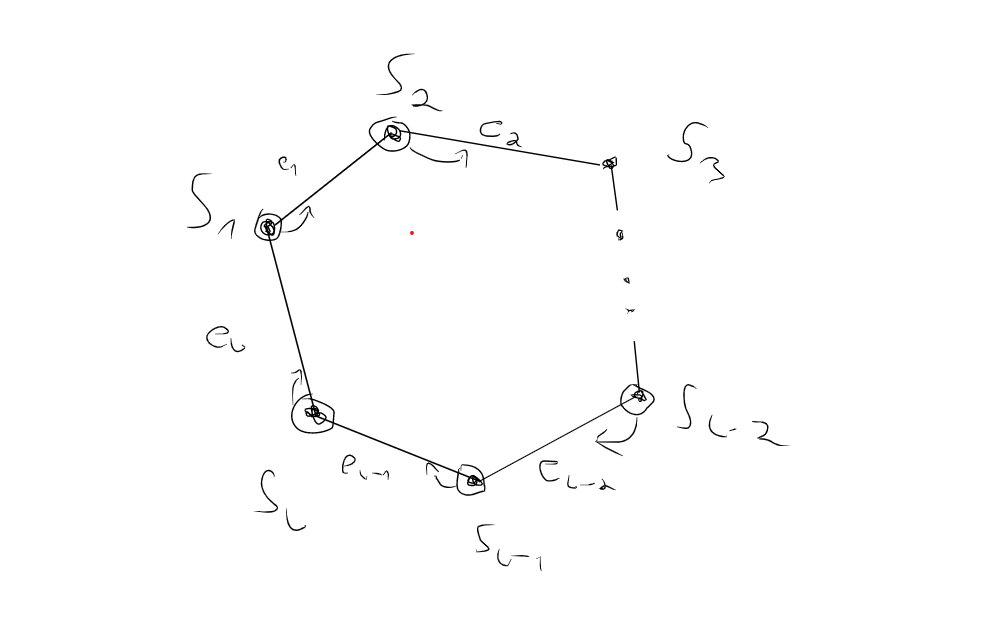
\includegraphics[scale=0.5]{boruvka} 
	\end{center}
	Jak widać na powyższym rysunku skoro \( e_2 \) zostało dołączone do \(S_2\) zamiast \(e_1\) to 
	\(c(e_1) > c(e_2)\). Kontynuując to rozumowanie dla każdego wierzchołka otrzymujemy nierówność
	\[ c(e_1) > c(e_2) > ... > c(e_{l-1}) > c(e_l) > c(e_1) \]
	Z której wynikałoby, że \( c(e_1) > c(e_1) \), więc mamy sprzeczność.
\end{enumerate}

W obu przypadkach otrzymaliśmy sprzeczność, czyli cykl nie mógł powstać.

\newpage
\noindent
\textbf{Zadanie 6} Jak zmodyfikować algorytm Boruvki, by działał również w grafach, w których jakieś krawędzie mają takie same wagi?
\vskip 0.5cm

Wystarczy, że przed uruchomieniem algorytmu posortujemy wagi krawędzi i do powtarzających się wag
dodamy różne, małe epsilony, nie zmieniające kolejności krawędzi w sortowaniu, a pozwalające ustalić porządek wśród takich samych wag i sprawiające że nie będą już one równe.

Następnie stosujemy algorytm Boruvki, wiemy, że dla różnych wag algorytm znajdzie MST. Odwracamy teraz proces dodawania epsilonów. Nie mógł on mieć wpływu na wagę wyjściowego drzewa, gdyż jedynie nadaliśmy nowy priorytet krawędziom, między którymi wybór jest dla nas i tak bez znaczenia, bo mają te same wagi.
\vskip 0.5cm
\noindent
\textbf{Zadanie 10} W pewnej grupie muzykujących osób Ania gra na skrzypcach, harfie, kontrabasie i wiolonczeli, Bartek gra na harfie i fortepianie, Cezary gra na fortepianie, Dąbrówka gra na harfie i Elwira gra na kontrabasie, skrzypcach, wiolonczeli i harfie. \\
Chcieliby zagrać utwór na fortepian, skrzypce, wiolonczelę, kontrabas i harfę. Czy uda im się dobrać skład?
\vskip 0.5cm

Dla lepszego zobrazowania, możemy narysować reprezentację tych relacji za pomocą grafu dwudzielnego.

\begin{center}
	\usetikzlibrary{positioning}
	\begin{tikzpicture}[
	roundnode/.style={circle, draw=black!60, fill=white!5, very thick, minimum size=7mm},
	roundnoder/.style={circle, draw=red!60, fill=white!5, very thick, minimum size=7mm}
	]
	%Nodes
	\node[roundnoder]      (ania)                              {A};
	\node[roundnode]       (bartek)       [below=of ania]      {B};
	\node[roundnode]       (cezary)       [below=of bartek]    {C};
	\node[roundnode]       (dabrowka)     [below=of cezary]    {D};
	\node[roundnoder]      (elwira)       [below=of dabrowka]  {E};
	\node[roundnode,right=7cm of ania]   (forte)              {F};
	\node[roundnoder]      (skrzypce)     [below=of forte]     {S};
	\node[roundnoder]      (wiol)         [below=of skrzypce]  {W};
	\node[roundnoder]      (kontr)        [below=of wiol]      {K};
	\node[roundnode]       (harf)         [below=of kontr]     {H};

	%Lines

	\draw[-, color=red] (ania.east) -- (skrzypce.west);
	\draw[-] (ania.east) -- (harf.west);
	\draw[-, color=red] (ania.east) -- (kontr.west);
	\draw[-, color=red] (ania.east) -- (wiol.west);
	
	\draw[-] (bartek.east) -- (harf.west);
	\draw[-] (bartek.east) -- (forte.west);
	
	\draw[-] (cezary.east) -- (forte.west);
	
	\draw[-] (dabrowka.east) -- (harf.west);
	
	\draw[-, color=red] (elwira.east) -- (skrzypce.west);
	\draw[-] (elwira.east) -- (harf.west);
	\draw[-, color=red] (elwira.east) -- (kontr.west);
	\draw[-, color=red] (elwira.east) -- (wiol.west);
	\end{tikzpicture}
\end{center}

Pytanie zatem jest o skojarzenie doskonałe, a z warunku Halla wiemy, że jest ono możliwe w grafie dwudzielnym tylko wtedy kiedy dla każdego \( A' \subseteq A \) zachodzi \( |N(A')| \geq |A'| \), oraz dla każdego \(B' \subseteq B\) zachodzi \( |N(B')| \geq |B'| \). Niech \(A\) będzie zbiorem osób, a \(B\) zbiorem instrumentów.

Zauważamy, że wtedy istnieje podzbiór \(B'\) zbioru \( B \) równy \( \{S,W,K\}\) (na rysunku, zaznaczony na po prawo na czerwono), taki że \( N(B') = \{A,E\} \), czyli \( |N(B')| < |B'| \), więc z warunku Halla wnioskujemy, że skojarzenie doskonałe nie może tutaj istnieć.

\end{document}